%--------------------------HOLE-------------------------------
% Что это?
% Это файл с простым текстом( выводы, описание чего-либо), который редактируются вручную.
% Описание (для чего файл):
% Hole number:4
\clearpage

\subsubsection{Система с переменной структурой со скользящим видом движения} \label{sub2}
Для выполнения данного пункта оставим прошлую модель в Matlab Simulink на рис.\ref{fig:sim_variable_structure1}.
Коэффициенты были подобраны таким образом, что $k_2=-k_1$. Коэффициенты указаны в табл.
\ref{tab:tab3}.

Изменим наше условие переключения между регуляторами. Таким образом математическая форма записи описанного ранее алгоритма управления \eqref{eq:eq3} примет вид \eqref{eq:eq4}.
\begin{equation} \label{eq:eq4}
\left\{ 
\begin{aligned}
\text{\"{x}}+k_1\,k\,\text{x}=0&,\text{x(\.{x}}+\tau\,\text{x})>0, \\
\text{\"{x}}-k_1\,k\,\text{x}=0&,\text{x(\.{x}}+\tau\,\text{x})<0.
\end{aligned}
\right.
\end{equation}

Два регулятора по-прежнему являются неустойчивыми. Один регулятор должен обеспечить движение изображающей точки по фазовой траектории типа «седло», а второй – по фазовой траектории типа «центр».

\begin{wraptable}{r}{0.5\linewidth}
	\caption{ Таблица параметров.} \label{tab:tab3}
	\begin{tabular}{|c|c|c|c|c|c|c|}
		\hline
		номер & $k_1$ & $k_2$ & $x_0$ & $y_0$ & $\tau_1$ & $\tau_2$ \\ \hline
		1&\multirow{3}{*}{1} &  \multirow{3}{*}{-1} & 0 & 0 &\multirow{3}{*}{3.74}&\multirow{3}{*}{0.935}\\ \cline{1-1} \cline{4-5} 
		2& & & 0.1 & 0.1 &&\\ \cline{1-1} \cline{4-5}
		3& & & 0.2 & 0.2 &&\\ \hline
	\end{tabular}
\end{wraptable}
В этом случае линиями раздела между областями действия регуляторов
будут ось ординат и наклонная прямая на фазовой плоскости, определяемая
выражением \.{x}=-$\tau\,$x, называемая \textbf{линией скольжения}. 
Также имеется \textbf{сепаратриса седловой траектории} с отрицательным наклоном, определяемая уравнением  \eqref{eq:eq5}.
\begin{equation}\label{eq:eq5}
\text{\.{x}}=-\sqrt{k}\,\text{x}
\end{equation}

В общем случае движение изображающей точки в зависимости от значения $\tau$ будет происходить по разным траекториям. Из расчетов видно $\sqrt{k}\hm{=}1.871$ .

Если взять $\tau\hm{=}\tau_1\hm{=}2\,\sqrt{k}\hm{=}3.74$, т.е. $\tau>\sqrt{k}$ в 2 раза, то мы будем наблюдать 
колебательный процесс рис.\ref{fig:variable_structure2_tau1}, в этом случае скольжения не наблюдается. То что процесс колебательный, мы можем видеть на рис.\ref{fig:variable_structure2_sys_tau1}.


\begin{figure}[!h]\centering	
	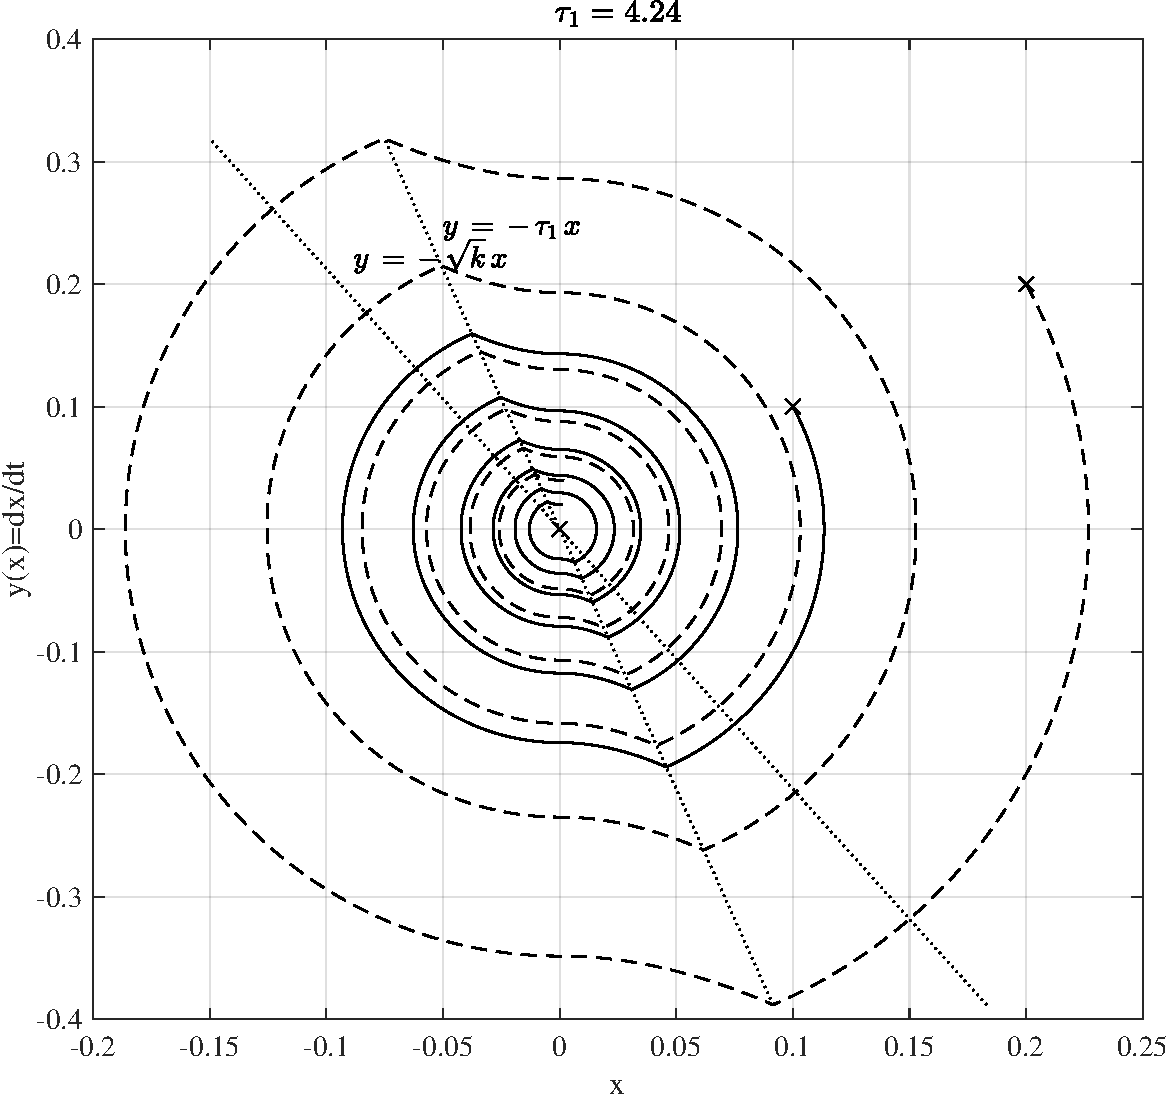
\includegraphics[width=0.7\linewidth]{images/variable_structure2_tau1}
	\caption{ Фазовые траектории для системы с переменной структурой с разными начальными условиями($\tau_1$).}\label{fig:variable_structure2_tau1}
\end{figure}
\begin{figure}[!h]\centering
	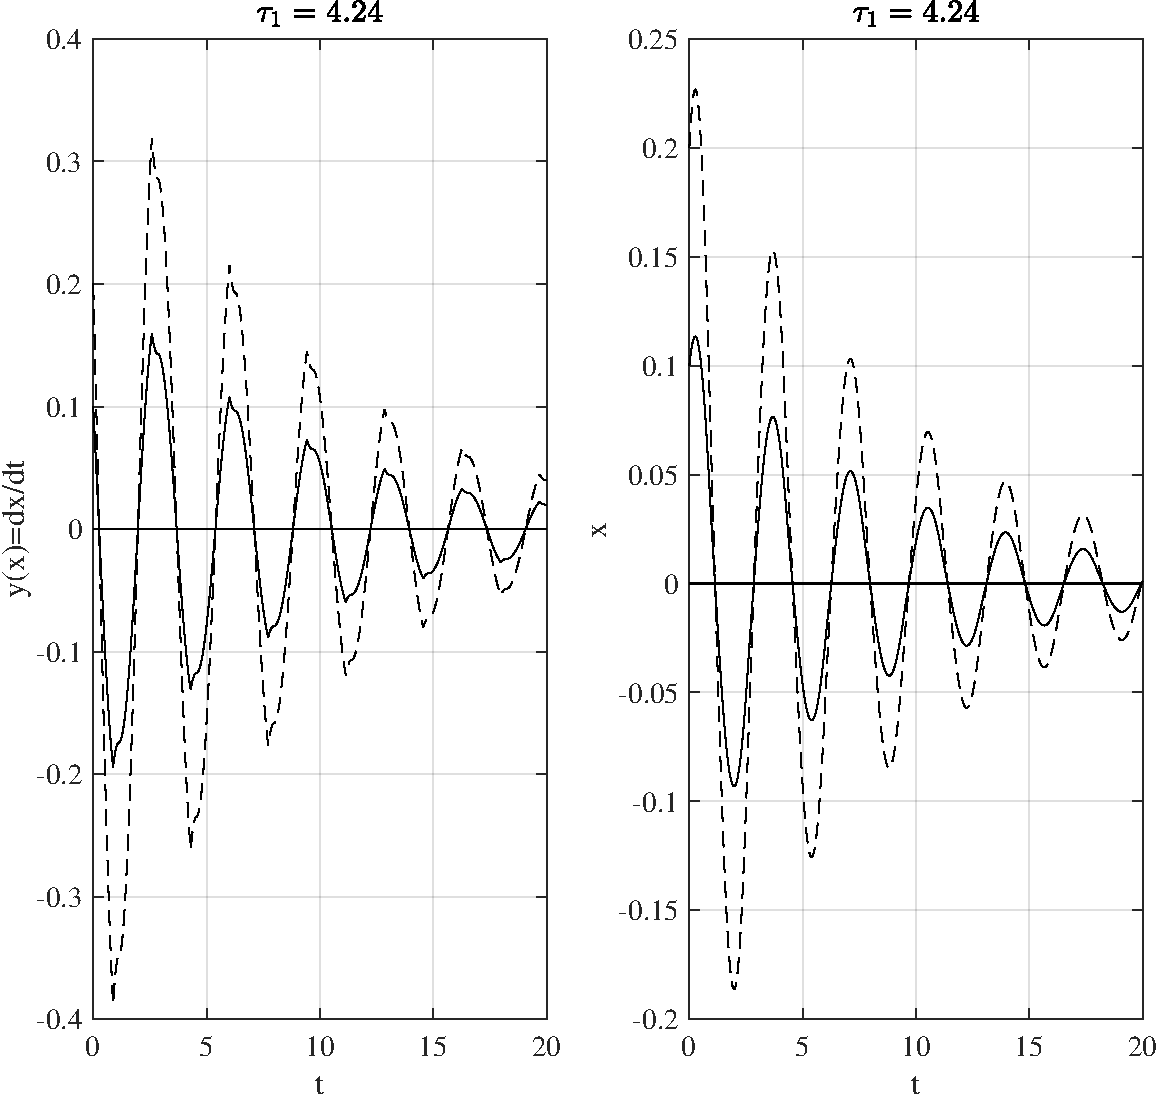
\includegraphics[width=0.7\linewidth]{images/variable_structure2_sys_tau1}
	\caption{ Графики изменения переменных состояния($\tau_1$).}\label{fig:variable_structure2_sys_tau1}
\end{figure}
\clearpage
Если взять $\tau\hm{=}\tau_1\hm{=}\sqrt{k}/2\hm{=}0.935$, т.е. $\tau<\sqrt{k}$ в 2 раза, то мы будем наблюдать 
апериодический процесс рис.\ref{fig:variable_structure2_tau2}, в этом случае движение
изображающей точки  происходит с одним переключением, после чего наблюдается скольжение вдоль прямой линиии  к началу
координат. То что процесс апериодический, мы можем видеть на рис.\ref{fig:variable_structure2_sys_tau2}.

\begin{figure}[!h]\centering
	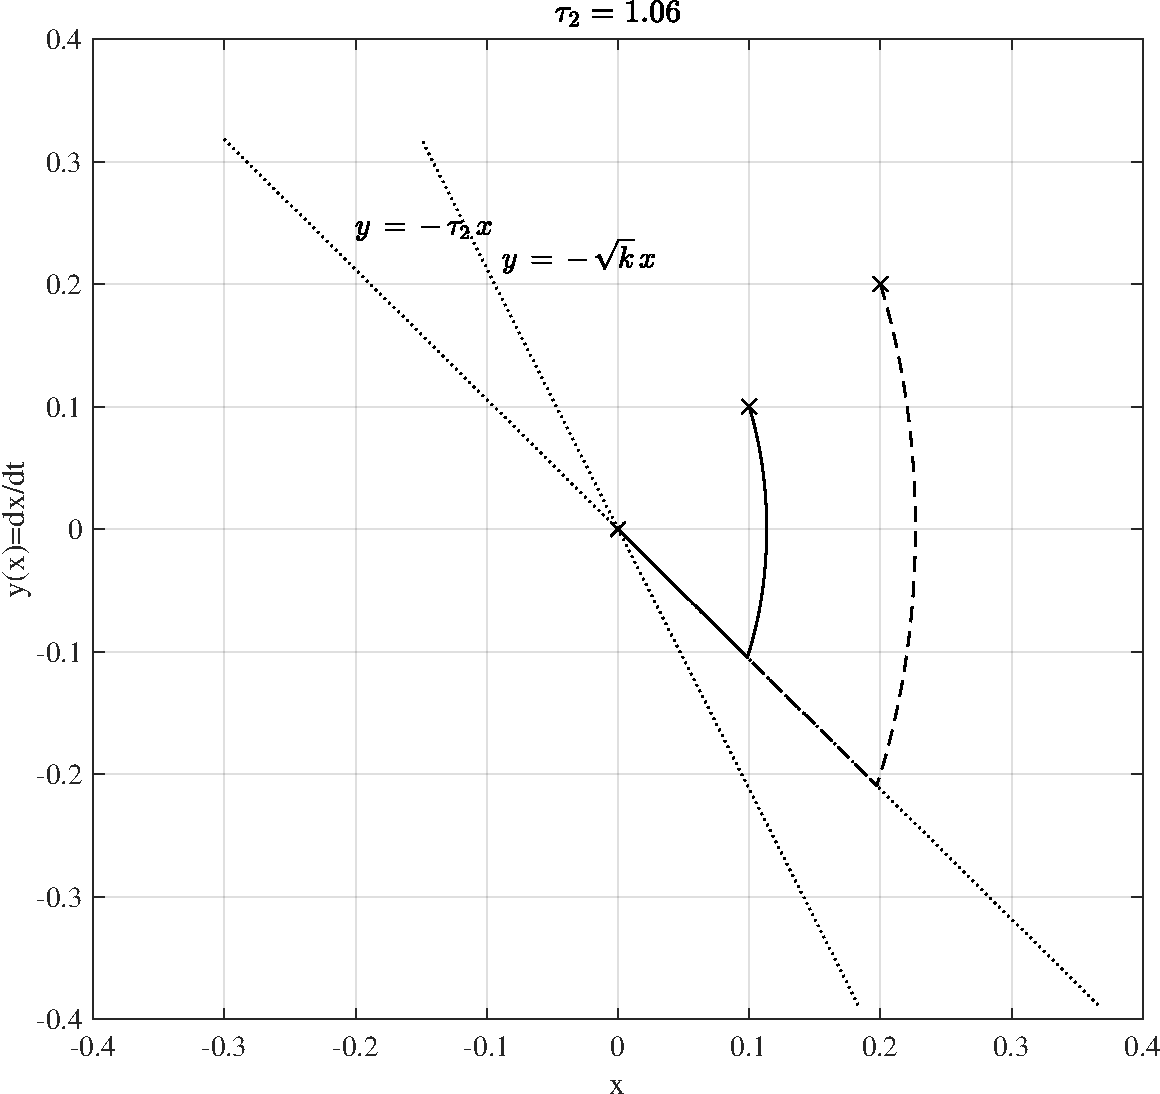
\includegraphics[width=0.7\linewidth]{images/variable_structure2_tau2}
	\caption{ Фазовые траектории для системы с переменной структурой с разными начальными условиями($\tau_2$).}\label{fig:variable_structure2_tau2}
\end{figure}
\begin{figure}[!h]\centering
	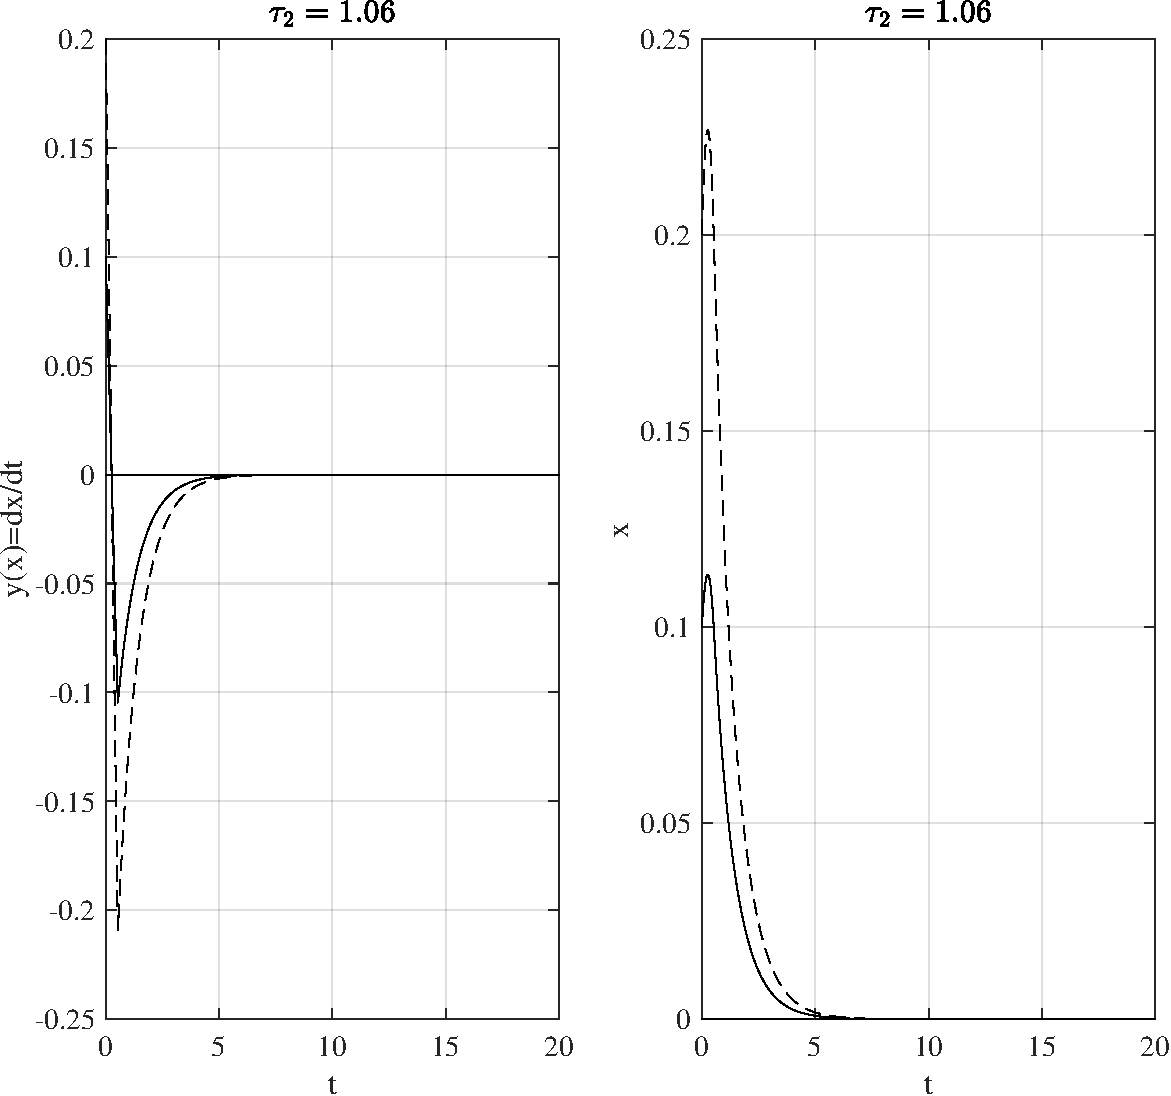
\includegraphics[width=0.7\linewidth]{images/variable_structure2_sys_tau2}
	\caption{ Графики изменения переменных состояния($\tau_2$).}\label{fig:variable_structure2_sys_tau2}
\end{figure}
Из пункта \ref{sub2} можно сделать вывод: 
\begin{enumerate}
	\item 
	Что введя новый закон переключения и имея два неустойчивых регулятора, причём один регулятор  обеспечивает движение изображающей
	точки по фазовой траектории типа «седло», а второй – по фазовой траектории
	типа «центр», можно созданием системы с переменной структурой добиться устойчивости системы в целом и получить режим, позволяющий привести изображающую точку в начало координат за
	минимальное число переключений, устранить колебательные процессы.
	\item
	Время протекания процесса при скользящем режиме уменьшилось по сравнению с другими режимами (это видно на рис.\ref{fig:variable_structure2_sys_tau2}).
	\item 
	Для данного примера скользящий режим будет выполняться только при $\tau<\sqrt{k}$.
\end{enumerate}

Вывод: применение систем с переменной структурой  со скользящим режимом позволяет получить высокое быстродействие, т. е. протекание процессов за минимальное время  и при отсутствии колебаний выходных координат в установившихся режимах.